\documentclass[11pt]{article}

\usepackage{pdflscape}
\usepackage{graphicx}
\usepackage[hidelinks]{hyperref}

\begin{document}

\begin{titlepage}
	\begin{center}
		
		\begin{figure}[t]
			\centering
			
\includegraphics[width=350px]{../Images/UP_Logo.png}
		\end{figure}
		
		% Title
		\textsc{\large } \\ 
		\vspace{2cm}
		\textbf{\Huge IMY 310 Project  \\
			Project Plan \\
			(Phase 1)} \\ 

		\textsc{\large } \\ 
		\vspace{0.75cm}

		\textbf{\Large AgriSales Magazine} \\ 
		
		\begin{flushright} \large
			Azhar Mohungoo \emph{12239799} \newline
			Daniel Malangu \emph{} \newline
			Kudzai  	\emph{} \newline
			\newline
			Group Name  \emph{} \newline
			\end{flushright}
		%\end{minipage}
		
	\end{center}
\end{titlepage}


\tableofcontents

\newpage

\section{Needs Identification}

There are people in the agriculture business that are in need of equipment. Some people do not know of places where to acquire the equipment they need, while others have equipment that is no longer of use to them for various reasons. Rather than searching for equipment at many different places, AgriSales aims to create a centralised market for people in this field to buy and sell equipment in the form of a website. And for people that do not have Internet access, AgriSales issues a magazine where new and used products are advertised.
\\ \\
The folowing are just some of the identified problems with the website:

\subsection{Functionality flaws: }

\begin{itemize}
	\item No proper way of contacting the owner of equipment other than a celphone number. Owner also has no way of contacting you back if you are not available on your cellphone.
	\item After an equipment has been sold, there is no way of making sure that the advertisement will be removed unless the seller removes it manually.
\end{itemize}

\subsection{Design flaws: }

\begin{itemize}
	\item The Login Form pops up and over other items on the page and doesn’t pop away.
	\item The website does not accommodate screens of different sizes, the design does not accommodate different devices.
	\item Advertisments flash and change which draws the users attention away from them.
	\item Menu has a missing options after you have logged in as an registered user.
	\item Some of the buttons have labels that are vague in their description, and you don’t intrusively know what pressing them will lead to.
	\item When you're trying to sell equipment the forms have missing inputs boxes.
	\item Sidebar menu just dissappears when you click on the profile link.
	\item A very useless attempt at animation in the form of a tractor on the home page.
	\item Back button is not part of the footer, just strangely placed at the top of the page.
\end{itemize}

\section{User Identification}

The user base are people that are invested in the agriculture and construction industry. It is aimed at people that are looking to buy or sell construction and commercial equipment. A subscription allows users that want to observe the market in order to stay up to date on the latest products, the current price ranges, and sales on equipment.
\\ \\
Our user groups include the following:

\begin{itemize}
	\item Buyers: Users who are looking to purchase equipment.
	\item Sellers: Users who are looking to dispose of their used equipment.
	\item Browsers: Users who look through the equipment which they can potentially buy.
\end{itemize}

\section{User Needs}

\begin{itemize}
	\item Users should be able to search for a product by name, model, price etc.
	\item Users who wish to sell their equipment, should be able to post an image of their product(s), either on the website or in the magazine, or both.
	\item Users who wish to buy or sell a product(s), should be able to register onto the website, in order to complete such action, except for viewing of equipement or contacting the owner of an equipement.
	\item Users should be able to subscribe and receive notifications from the website or new installments of the magazine.
\end{itemize}

\section{Conceptual Design}

	\subsection{Home Page}
	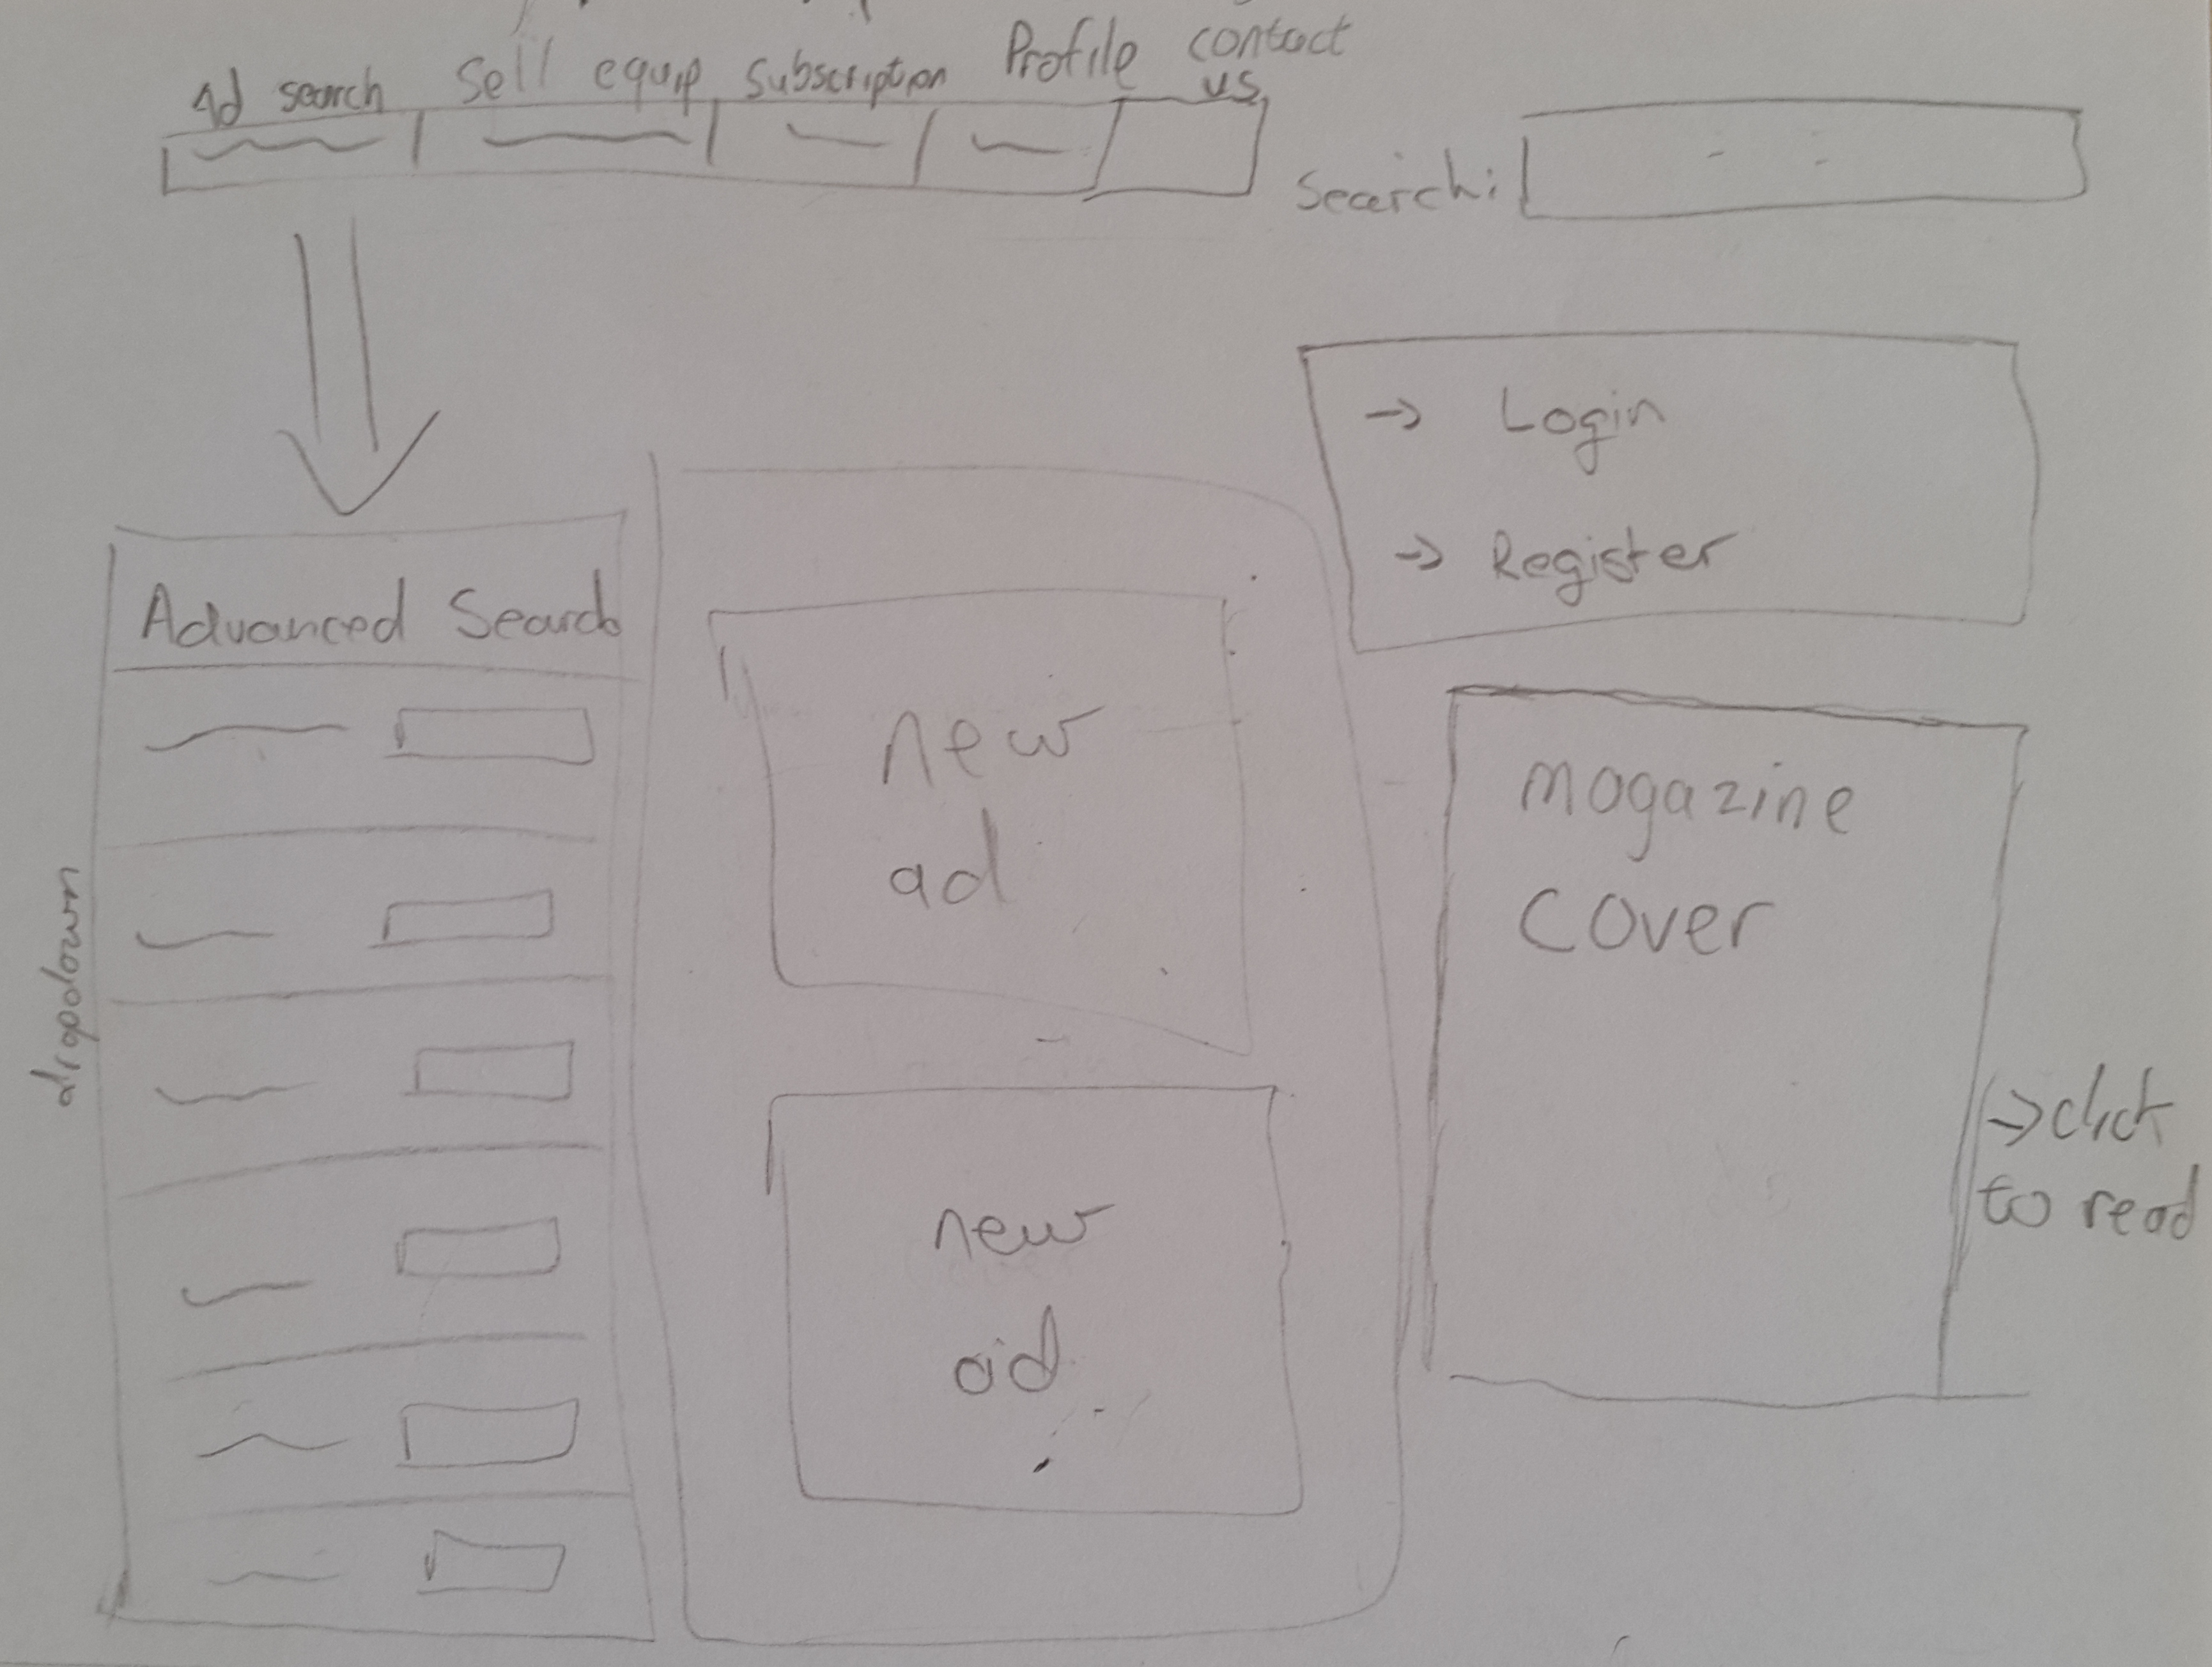
\includegraphics[width=\textwidth]{../Images/HomePage.jpg} \\
	
	\begin{itemize}
	\item We added the simple search bar, so that the user can easily search at a faster rate. We changed the layout so that it's less cluttered so the user can see the different options. Advance search is a now dropdown menu. Main page now focuses on latest adverts sorted cronologically. The magazine cover has been reduced in size and moved to the right side. The menu bar has been frozen to the top of the page so that when users scroll down, it's still be visible, for ease of use. \newpage
	\end{itemize} 
	
	\subsection{Login Page} 
	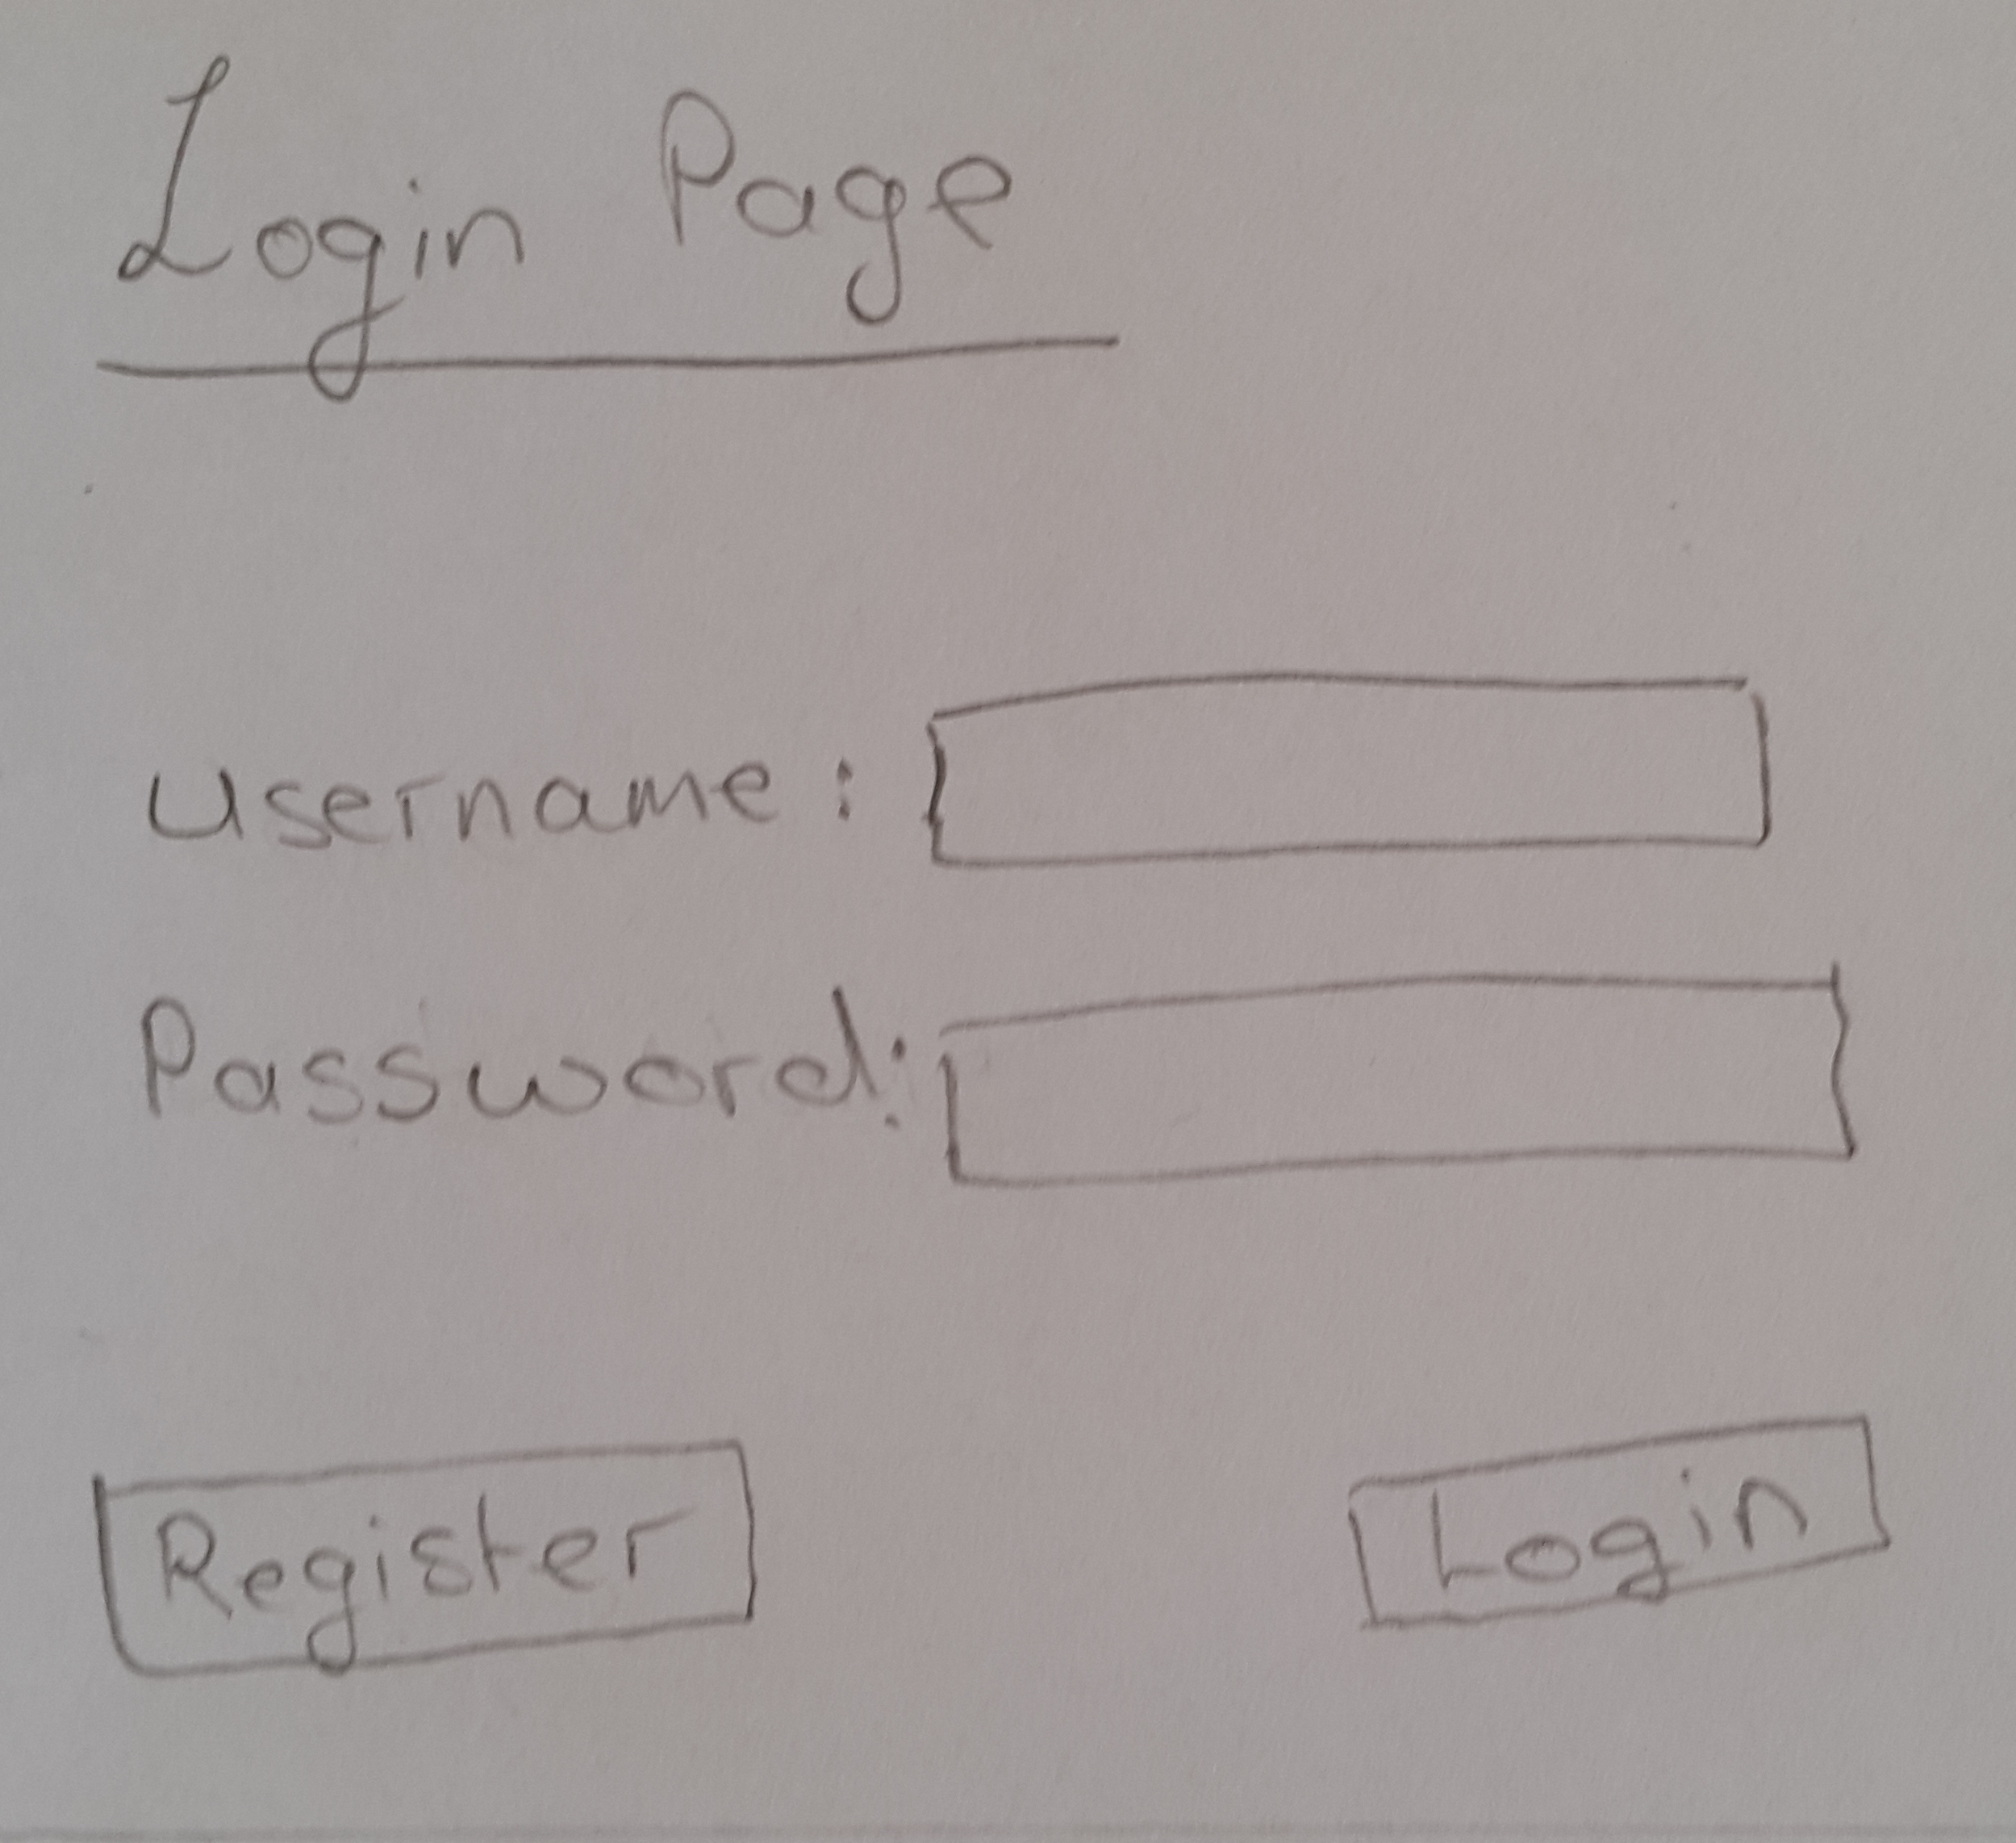
\includegraphics[width=\textwidth]{../Images/LoginPage.jpg} \\
	
	\begin{itemize}
		\item Login page has been separated from the homepage to avoid making the homepage overcrowded with information, to decrease the amount of options displayed to the user on the homepage. \newpage
	\end{itemize} 
	
	\subsection{View Adverts}
	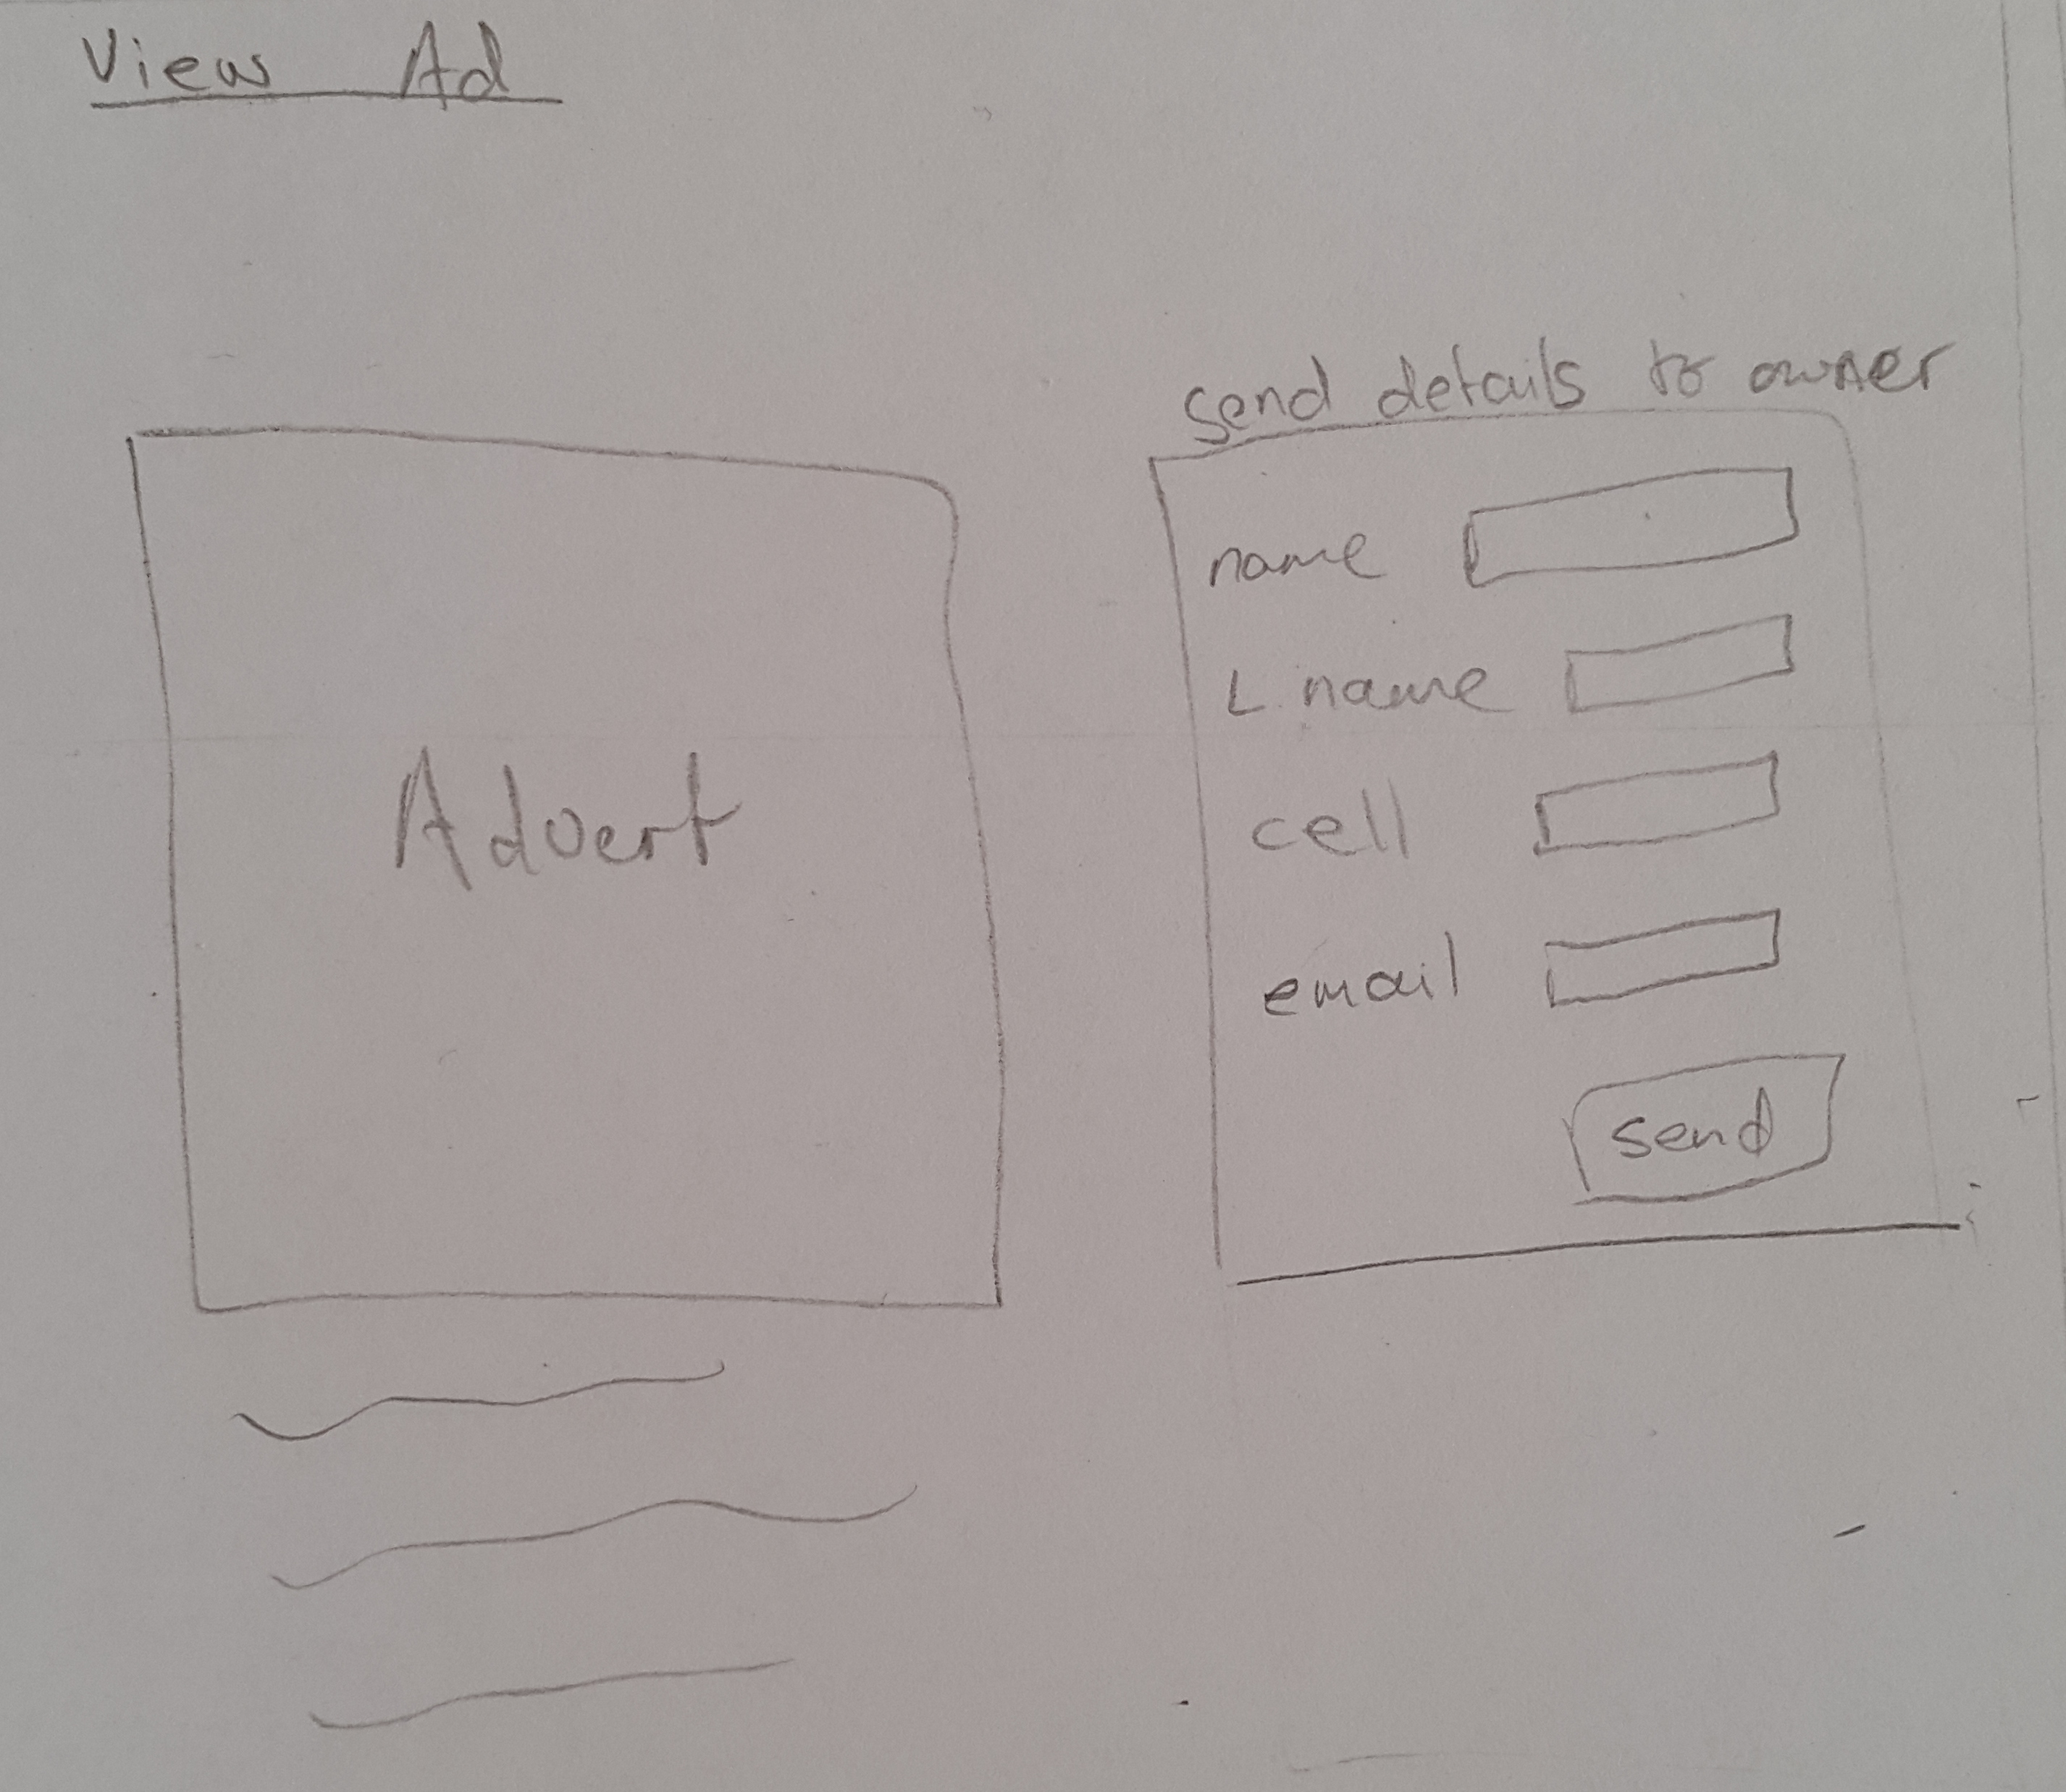
\includegraphics[width=\textwidth]{../Images/ViewAdverts.jpg} \\
	
	\begin{itemize}
		\item View adverts has been given it's own page so that the user can distincly view one advert and the equipment's it's details at a time and they will now be able to contact the owner by sending their own details via email. \newpage
	\end{itemize}
	
\end{document}
